\documentclass{book}
\usepackage{mathalpha}
\usepackage[utf8]{inputenc}
\usepackage{cancel}
\usepackage[margin=2cm, a4paper]{geometry}
\usepackage{amsmath}
\usepackage{amssymb}
\usepackage{gensymb}
\usepackage{graphicx}
\usepackage{hyperref}
\usepackage{pgfplots}
\usepackage{tikz}
\usepackage{pdfpages}
\usepackage{parskip}
\usepackage{polynom}
\usepackage{multirow}

\title{Physics}
\author{Lachlan Takumi Ikeguchi}

\begin{document}
\maketitle
\tableofcontents

\section{The purpose}
This document was written to be used as a summary to help revise the content covered in Physics.  For any inquiries, feedback, and further explanations, contact lachlanprivate@duck.com or through the discord server: \url{https://discord.gg/6P8rddkXFr}.  I encourage you to let me know of any topic I missed, how I could explain it better, or how it could be reworded or formatted to be more helpful in its purpose.  The goal of this document is to be a comprehensive summary of everything you need to know.

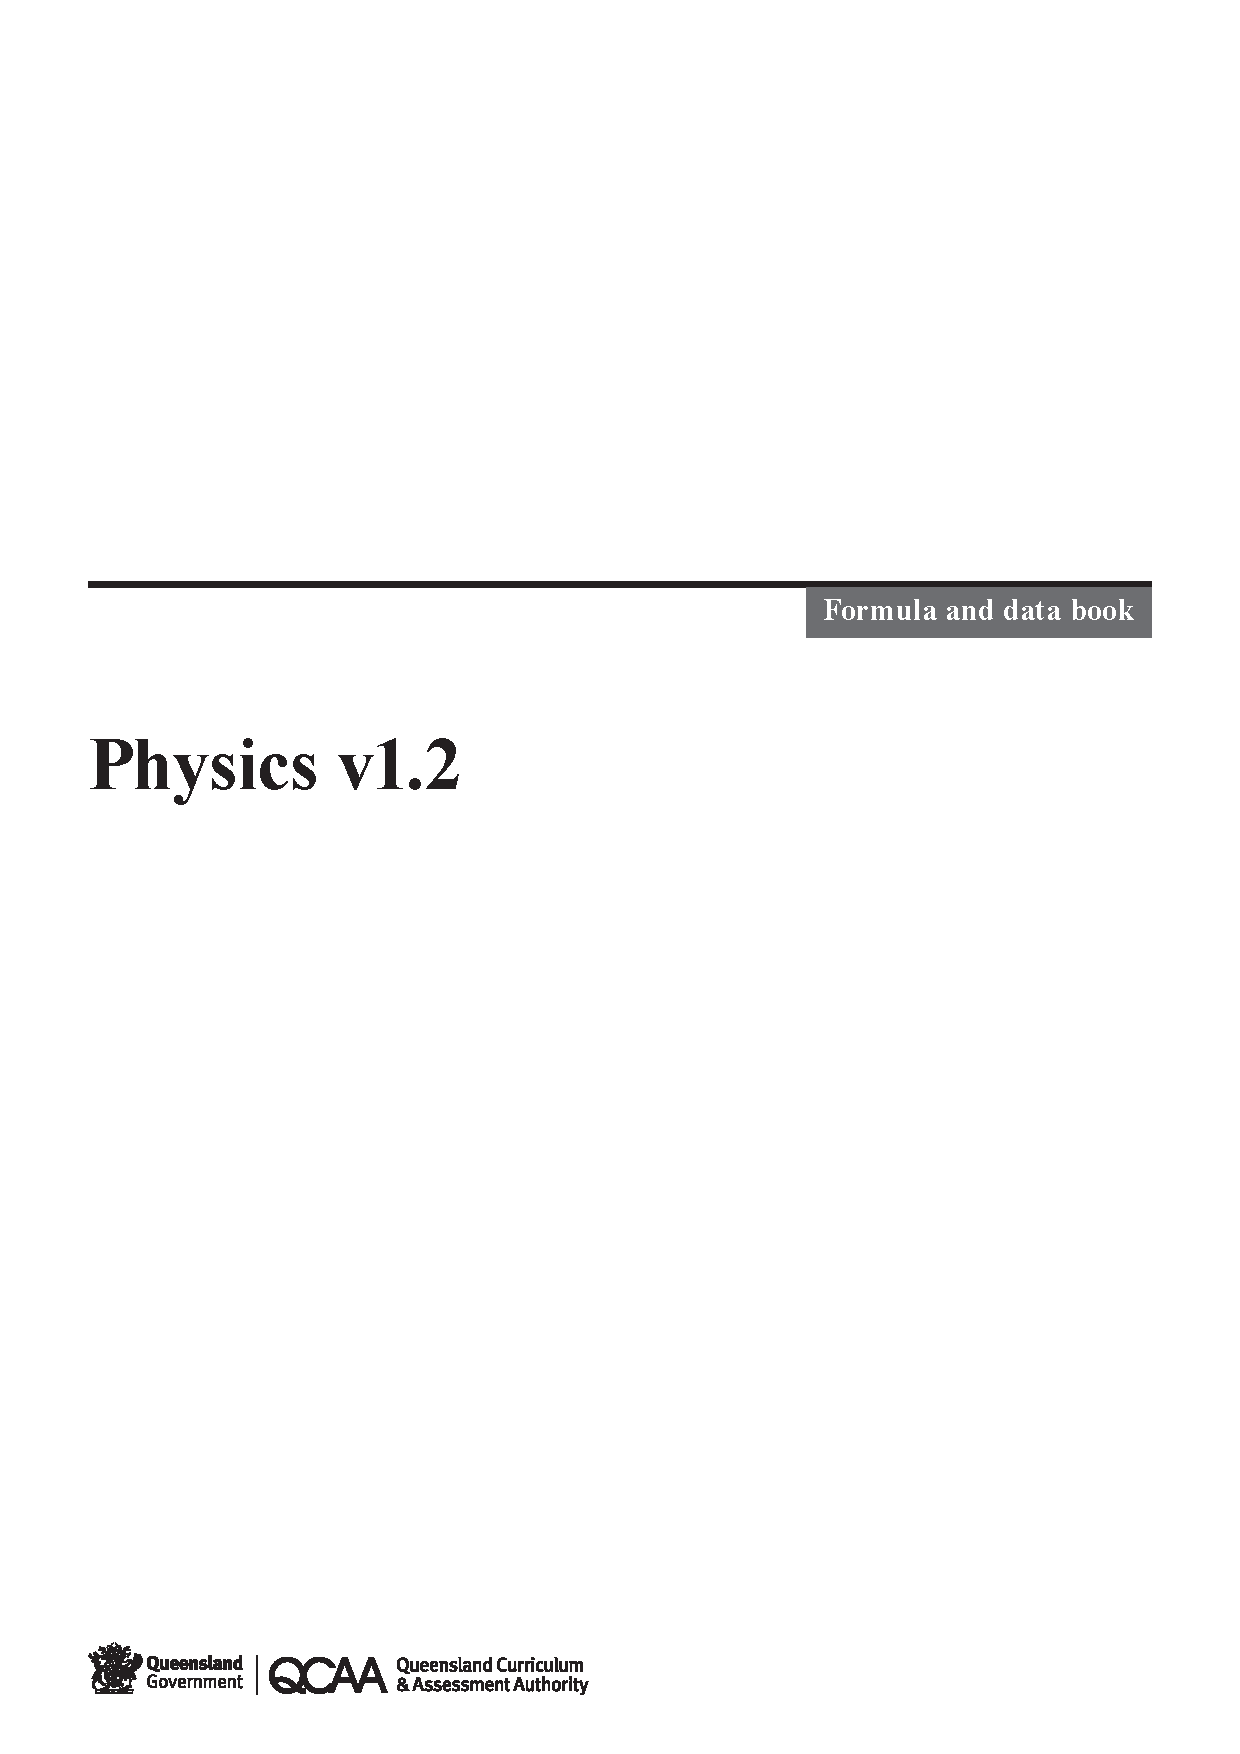
\includepdf[pages={1-9}]{./images/formula-book.pdf}

\chapter{Data}
\section{Measurement uncertainty}

\section{Error}

\chapter{Heating process}
\section{Definitions}
\subsection{Heat}
Heat is defined as the rate of transfer of internal energy.

\section{Kinetic particle model}

\section{Heat}

\section{Temperature}

\section{Specific heat capacity}

\section{Calorimetry}

\section{Specific latent heat}

\chapter{Radiation and nuclear reactions}


\chapter{Electrical circuits}

\chapter{Linear motion}

\chapter{Waves and Light}

\end{document}
